\documentclass[letterpaper,11pt]{article}
\usepackage{graphicx}
\usepackage{listings}
\usepackage[super]{nth}
\usepackage[hyphens]{url}
\usepackage{hyperref}
\usepackage{amsmath}
\usepackage[makeroom]{cancel}
\usepackage[table]{xcolor}
\usepackage{comment}
\usepackage[space]{grffile}

\lstset{
	basicstyle=\footnotesize,
	breaklines=true,
}

\begin{document}

\begin{titlepage}

\begin{center}

\Huge{Assignment 9}

\Large{CS 595:  Introduction to Web Science}

\Large{Fall 2013}

\Large{Shawn M. Jones}

\Large Finished on \today

\end{center}

\end{titlepage}

\newpage


\newpage
\section*{1}

\subsection*{Question}

\begin{verbatim}
1.  Create a blog-term matrix.  Start by grabbing 100 blogs; include:

http://f-measure.blogspot.com/
http://ws-dl.blogspot.com/

and grab 98 more as per the method shown in class.

Use the blog title as the identifier for each blog (and row of the
matrix).  Use the terms from every item/title (RSS) or entry/title
(Atom) for the columns of the matrix.  The values are the frequency
of occurrence.  Essentially you are replicating the format of the
"blogdata.txt" file included with the PCI book code.  Limit the
number of terms to the most "popular" (i.e., frequent) 500 terms,
this is *after* the criteria on p. 32 (slide 7) has been satisfied.
\end{verbatim}

\subsection*{Answer}

The script \verb+fetchFeeds.py+ shown in Listing \ref{lst:q1fetch} outputs a list of URIs that dereference to Atom feeds.  

This script uses a canned URI on line $54$ to acquire the next blog URI via the call on line $82$.  If it failed to acquire this URI, it sleeps for 5 seconds and tries again.  If successful, it then dereferences the URI using the function defined on line $12$.  This function returns the representation of the resource, as well as its URI after all redirects have been followed.  

If that is successful, it uses the function defined on line $21$ to extract the Atom URI from the blog's HTML.  If that is successful, it then tries to dereference the Atom feed URI, again acquiring the representation and the redirect-free version of the atom URI.  Then it tests the URI using the function defined on line $33$.  This function checks to ensure that the blog has at least 25 entries.  Attempts to ensure that the blog was English did not work well, as all Blogger pages use a character encoding of UTF-8, and detecting 'English' (maybe using a dictionary?) appeared to be outside the realm of this assignment.

Once the URI gets through all of those wickets, it is saved to a list, with the query string ``?max-results=1000'' appended.  This ensures that we get at most $1000$ entries from each blog, providing the maximum amount of data for the following questions.  Because all blogs come from Blogger, which has a consistent API, this query string works every time.

\lstinputlisting[frame=single,caption={Python script for fetching valid Atom feeds from Blogger},label=lst:q1fetch,captionpos=b,numbers=left,showspaces=false,showstringspaces=false,basicstyle=\footnotesize]{q1/fetchFeeds.py}

The script is run like so:
\begin{lstlisting}[frame=single]
./fetchFeeds.py > feedlist.txt
\end{lstlisting}

Once \verb+feedlist.txt+ exists, it can be used by Toby Segaran's \verb+generatefeedvector.py+\cite{pci}.  I only modified that script on line $59$ so that it could handle UTF-8 encodings for some of the blogs.  It is captured in Listing \ref{lst:appSegaran1} on page \pageref{lst:appSegaran1}.

The script \verb+eliminateWords.py+  shown in Listing \ref{lst:q1eliminate} takes in the \verb+blogdata1.txt+ file produced by \verb+generatefeedvector.py+ and removes the top N terms from it.

It does this by generating scores for each word by summing all of its frequencies across all blogs together.  Once it has those scores, it gets the top $n$ words.  It then determines the index of each of those words in the list.  Using these indices, it regenerates the format of \verb+blogdata.txt+, only printing out each column if it is an ``approved'' index.

The final file is saved to github as \verb+blogdata500.txt+ and is used for each subsequent question.

\lstinputlisting[frame=single,caption={Python script for eliminating words from blog data},label=lst:q1eliminate,captionpos=b,numbers=left,showspaces=false,showstringspaces=false,basicstyle=\footnotesize]{q1/eliminateWords.py}

\newpage

\section*{2}

\subsection*{Question}

\begin{verbatim}
2.  Create an ASCII and JPEG dendrogram that clusters (i.e., HAC)
the most similar blogs (see slides 12 & 13).  Include the JPEG in
your report and upload the ascii file to github (it will be too
unwieldy for inclusion in the report).
\end{verbatim}

\subsection*{Answer}

The script \verb+makeDendogram.py+, shown in Listing \ref{lst:q2script} uses Toby Segaran's \emph{clusters.py} \cite{pci} shown on page \pageref{lst:appSegaran2}.

\lstinputlisting[frame=single,caption={Python script for generating dendograms from the blog data captured in question 1},label=lst:q2script,captionpos=b,numbers=left,showspaces=false,showstringspaces=false,basicstyle=\footnotesize]{q2/makeDendogram.py}

It is run like so:
\begin{lstlisting}[frame=single]
./makeDendogram.py > ascii-dendogram.txt
\end{lstlisting}

The \verb+printclust+ function on line $16$ prints out the the dendogram, so shell redirection is used to save it.  The \verb+drawdendogram+ function on line $19$ saves a JPEG of the dendogram, which can be seen in Figure \ref{fig:q2dendogram}.

\clearpage
\begin{figure}[h]
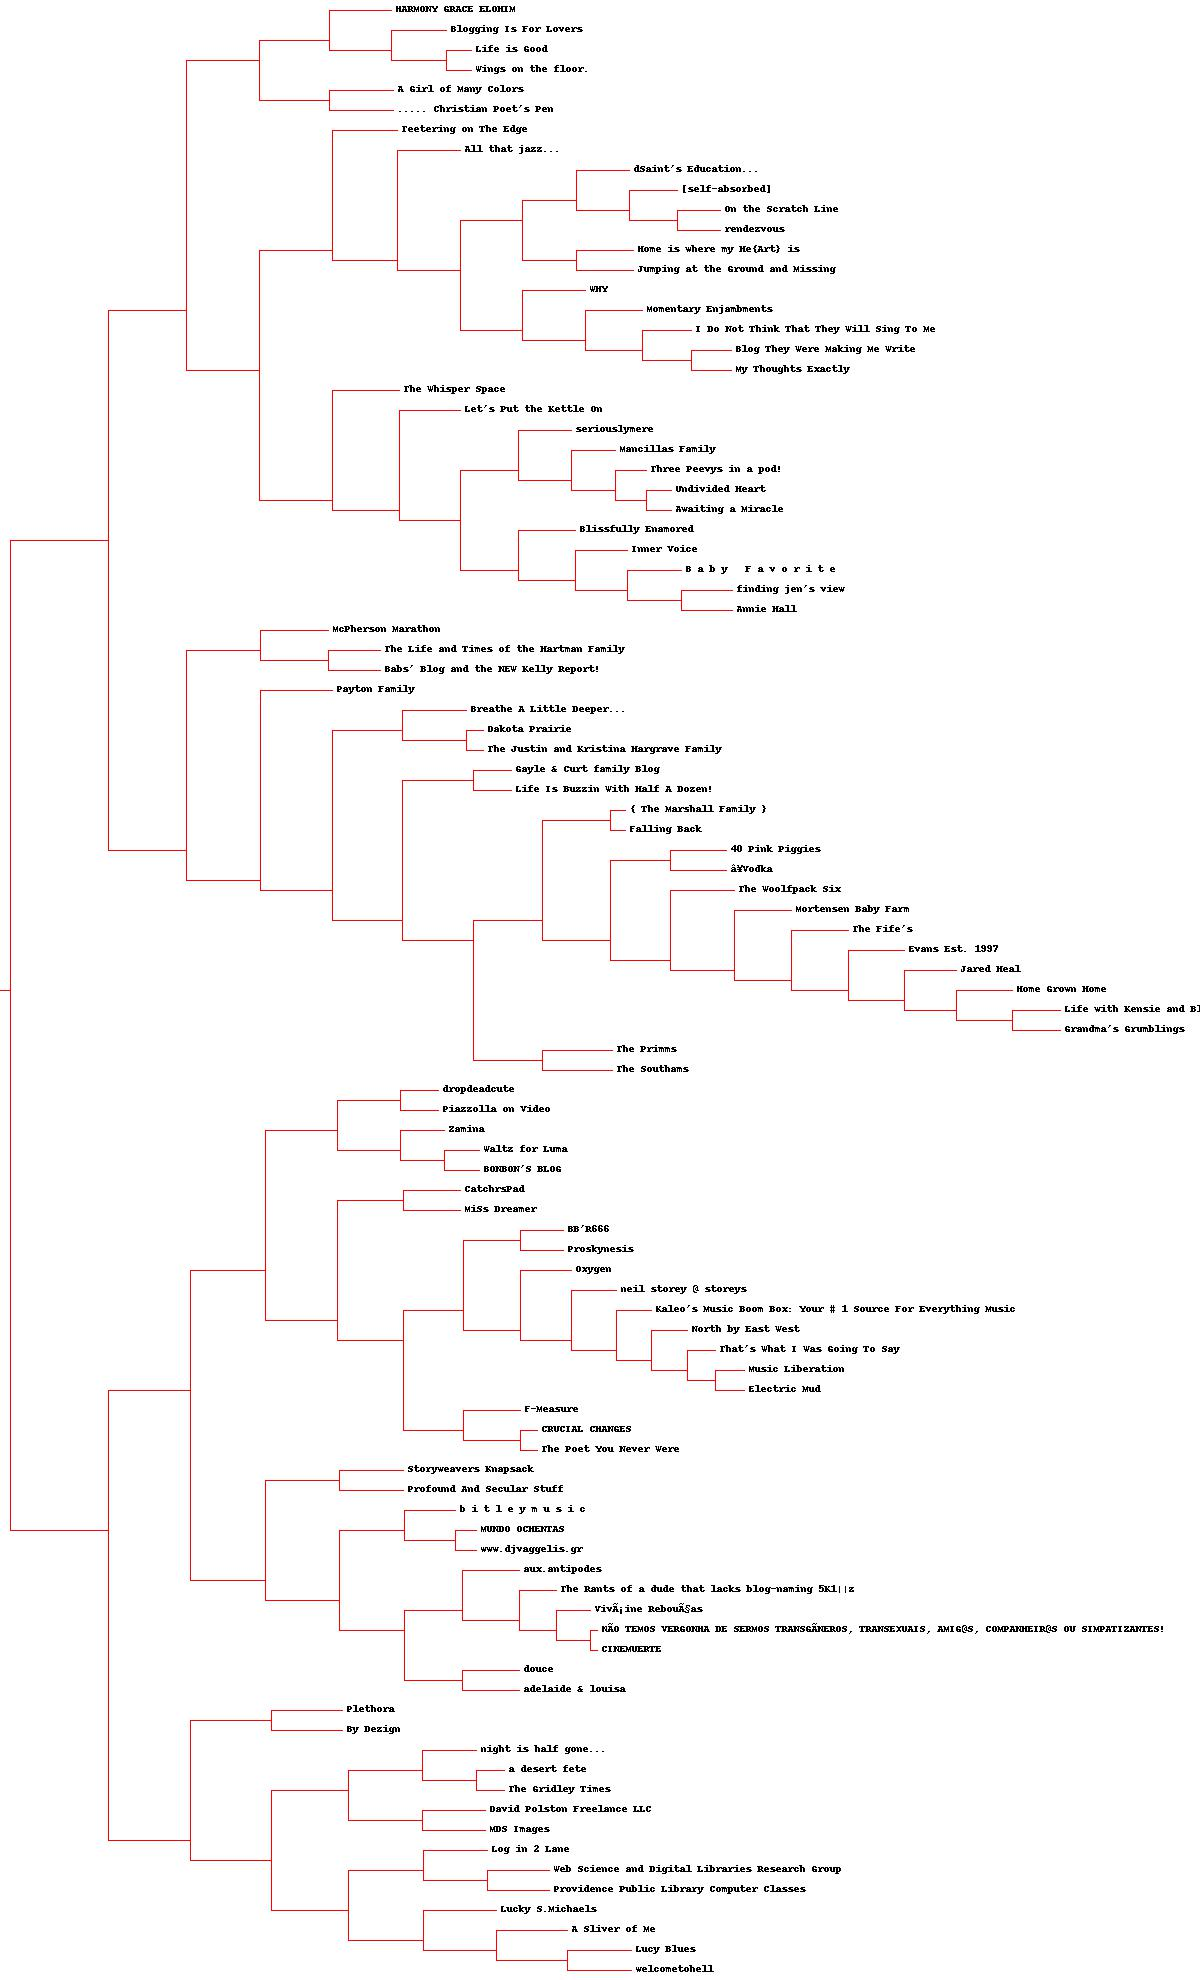
\includegraphics[scale=0.26]{q2/blogclust.jpg}
\caption{Dendogram produced by the \emph{makeDendogram.py} script}
\label{fig:q2dendogram}
\end{figure}

\clearpage
Unfortunately, it is difficult to see, but this dendogram shows that the blogs calculated to be most like \emph{F-Measure} are \emph{CRUCIAL CHANGES} and \emph{The Poet You Never Were}.  The blog calculated to be most like \emph{Web Science and Digital Libraries Research Group} is \emph{Providence Public Library Computer Classes}.

\clearpage

\section*{3}

\subsection*{Question}

\begin{verbatim}
3.  Cluster the blogs using K-Means, using k=5,10,20. (see slide 18).
How many interations were required for each value of k?
\end{verbatim}

\subsection*{Answer}

The blog clustering is performed by the script shown in Listing \ref{lst:q3script}, which makes use of Toby Segaran's \emph{clusters.py} \cite{pci} on page \pageref{lst:appSegaran2}., using the function \emph{kcluster} on lines $15$, $19$, and $23$.

\lstinputlisting[frame=single,caption={Python script for clustering the blogs using K-means, using k=5, 10, and 20},label=lst:q3script,captionpos=b,numbers=left,showspaces=false,showstringspaces=false,basicstyle=\footnotesize]{q3/makeClusters.py}

This script is run like so:

\begin{lstlisting}[frame=single]
./makeClusters.py
\end{lstlisting}

\newpage
From its output, we see how many iterations each value of $k$ produces.
\begin{lstlisting}[frame=single]
For k=5
Iteration 0
Iteration 1
Iteration 2
Iteration 3
Iteration 4

For k=10
Iteration 0
Iteration 1
Iteration 2
Iteration 3
Iteration 4
Iteration 5
Iteration 6
Iteration 7

For k=20
Iteration 0
Iteration 1
Iteration 2
Iteration 3
\end{lstlisting}

Thus, for $k=5$ we get $5$ iterations, for $k=10$ we get $8$ iterations, and for $k=20$ we get $4$ iterations.

\newpage

\section*{4}

\subsection*{Question}

\begin{verbatim}
4.  Use MDS to create a JPEG of the blogs similar to slide 29.  
How many iterations were required?
\end{verbatim}

\subsection*{Answer}

The blog space is generated using multidimensional scaling from the script \verb+makeMDS.py+ shown in Listing \ref{lst:q4script}, which makes use of Toby Segaran's \emph{clusters.py} \cite{pci} on page \pageref{lst:appSegaran2}, using the functions \emph{scaledown} on line $14$ and \emph{draw2d} on line $16$.

\lstinputlisting[frame=single,caption={Python script for generating a MDS from the blog data},label=lst:q4script,captionpos=b,numbers=left,showspaces=false,showstringspaces=false,basicstyle=\footnotesize]{q4/makeMDS.py}

Again, unfortunately the blog space produced does not fit well on a letter-sized page shown in Figure \ref{fig:q4MDS}.  According to this two-dimensional representation, the blog closest to \emph{F-Measure} is \emph{Piazzolla on Video}.  The blog closest to \emph{Web Science and Digital Libraries Research Group} is \emph{..... Christian Poet's Pen}.

Listing \ref{lst:q4output} shows the output from running this script, which took $253$ iterations on this run.

\clearpage
\begin{figure}[h]
\centerline{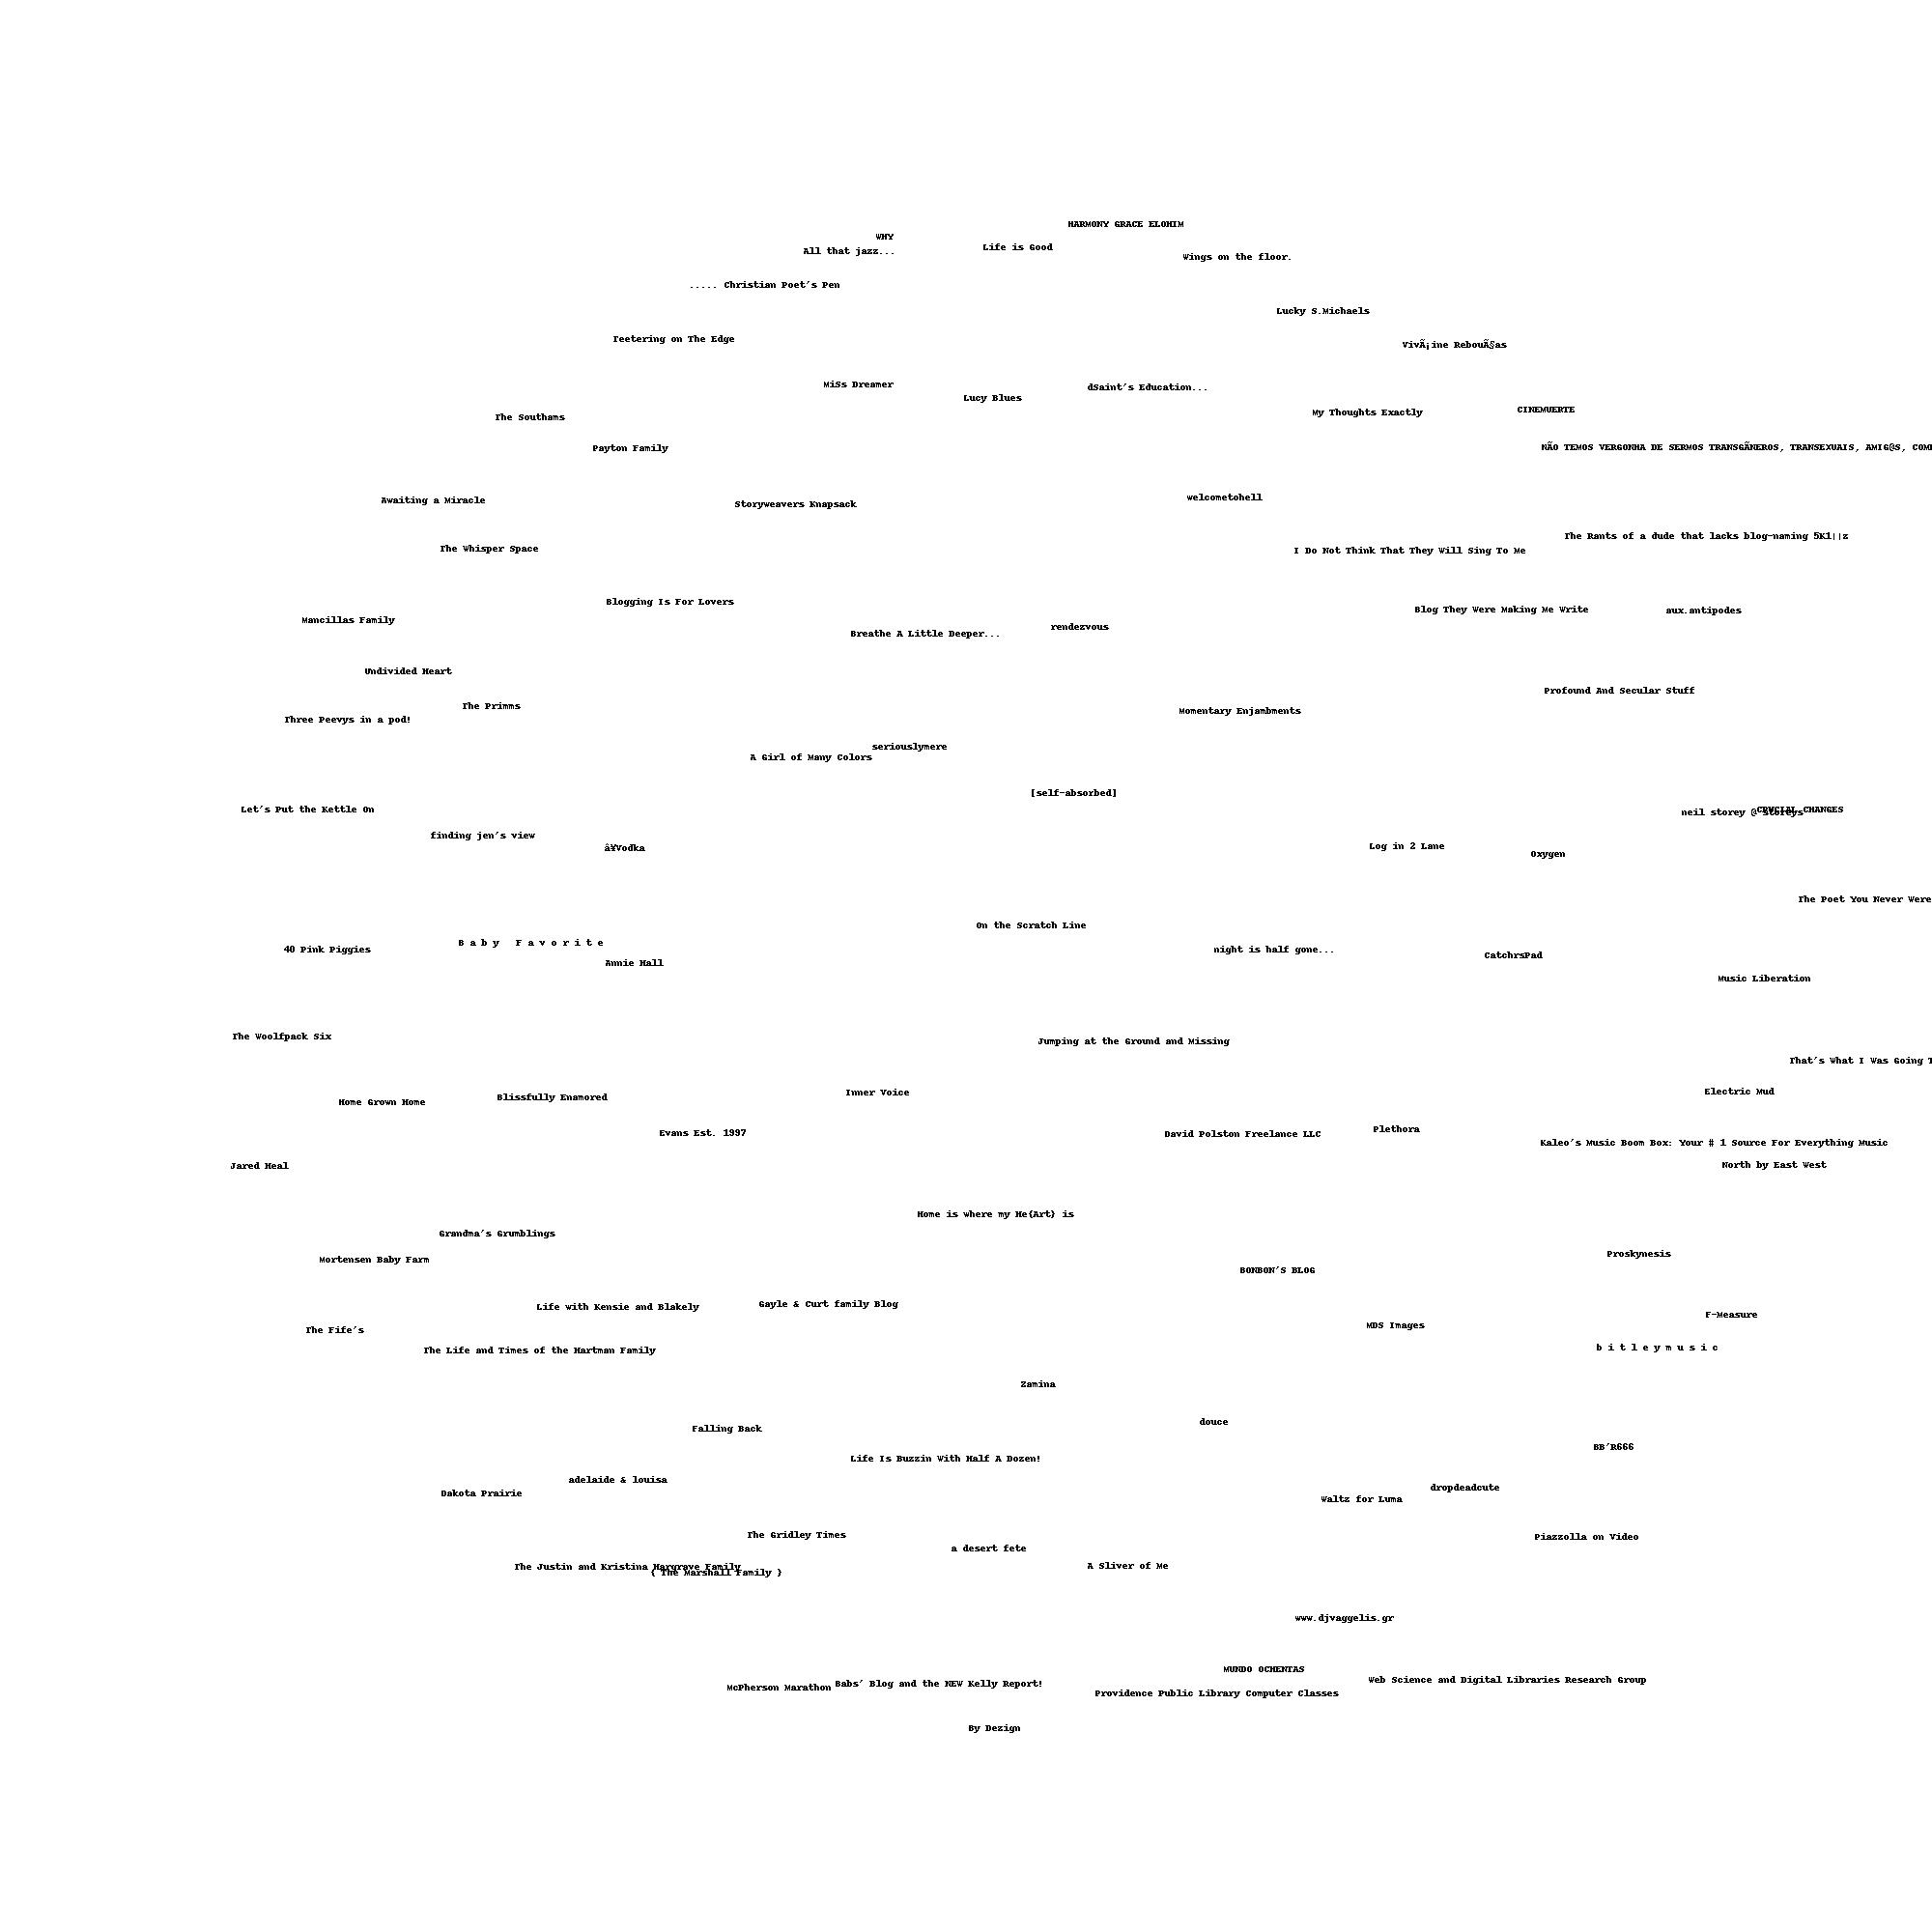
\includegraphics[scale=0.26]{q4/blogs2d.jpg}}
\caption{Blog space produced by the \emph{makeMDS.py} script}
\label{fig:q4MDS}
\end{figure}

\clearpage

\lstinputlisting[frame=single,caption={Output from script \emph{makeMDS.py}},label=lst:q4output,captionpos=b,numbers=left,showspaces=false,showstringspaces=false,basicstyle=\footnotesize]{q4/q4output.txt}

\clearpage

\newpage

\section*{5}

\subsection*{Question}

\begin{verbatim}
5.  Re-run question 2, but this time with proper TFIDF calculations
instead of the hack discussed on slide 7 (p. 32).  Use the same 500
words, but this time replace their frequency count with TFIDF scores
as computed in assignment #3.  Document the code, techniques,
methods, etc. used to generate these TFIDF values.  Upload the new
data file to github.

Compare and contrast the resulting dendrogram with the dendrogram
from question #2.

Note: ideally you would not reuse the same 500 terms and instead
come up with TFIDF scores for all the terms and then choose the top
500 from that list, but I'm trying to limit the amount of work
necessary.
\end{verbatim}

\subsection*{Answer}
Not attempted.


\clearpage
\appendix
\section{Segaran's \emph{generatefeedvector.py}}

\lstinputlisting[frame=single,caption={Segaran's \emph{generatefeedvector.py}, with small modification added on line 59 to handle UTF-8 encodings},label=lst:appSegaran1,captionpos=b,numbers=left,showspaces=false,showstringspaces=false,basicstyle=\footnotesize]{q1/generatefeedvector.py}

\clearpage
\section{Segaran's \emph{clusters.py}}

\lstinputlisting[frame=single,caption={Segaran's \emph{clusters.py}},label=lst:appSegaran2,captionpos=b,numbers=left,showspaces=false,showstringspaces=false,basicstyle=\footnotesize]{libs/clusters.py}


\clearpage
\bibliographystyle{acm}
\bibliography{references}

\end{document}